\begin{figure}
\makebox[\textwidth][c]{
\begin{tikzpicture}
\begin{axis}[%
width=0.8\textwidth,
xlabel={\# of assets},
ylabel={Exe Time (s)},
legend pos=north west,
title=\textbf{Average execution time with {$\epsilon=10^{-6}$}},
]
\addplot [color=blue,solid,mark=x,mark options={solid}]
  table[row sep=crcr]{%
%5	8.3		\\
%10	13.8		\\
%20	25.9		\\
%30	42.5		\\
%50	.088		\\
%75	.141		\\
100	.167	\\
200	.420	\\
300	.787 	\\
500	2.519  	\\
750	7.834		\\
1000 18.686		\\
1250 33.661 \\
%1500 55.57 \\
%2000 197.34 \\
};
\label{Subplot:exe_e6_exact}

\addplot [color=red,solid,mark=x,mark options={solid}]
  table[row sep=crcr]{%
%5	5.5		\\
%10	10.2		\\
%20	19		\\
%30	29.5		\\
%50	.0617		\\
%75	.104		\\
100	.122	\\
200	.374		\\
300	.803		\\
500	3.032	\\
750	10.84		\\
1000	 27.801	\\
1250 52.762\\
};
\label{Subplot:exe_e6_armijo}

\addplot [color=gr,solid,mark=x,mark options={solid}]
  table[row sep=crcr]{%
%5	8.3		\\
%10	13.8		\\
%20	25.9		\\
%30	42.5		\\
%50	.009		\\
%75	.019	\\
100	.010		\\
200	.039		\\
300	.091	\\
500	.399	\\
750	1.347		\\
1000 3.380		\\
1250 	6.470	\\
%2000 32.865 \\
};
\label{Subplot:exe_e8_snopt}
\addlegendentry{Optimal Step}
\addlegendentry{Armijo Step}
\addlegendentry{SNOPT}
\end{axis}
\end{tikzpicture}
}

\makebox[\textwidth][c]{
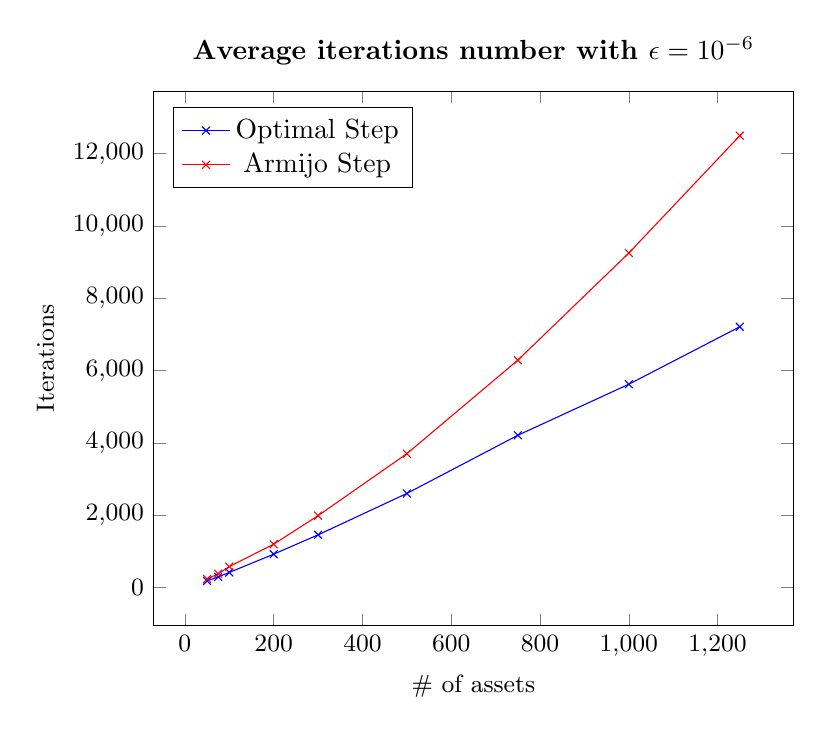
\begin{tikzpicture}
\begin{axis}[%
width=0.8\textwidth,
xlabel={\# of assets},
ylabel={Iterations},
scaled y ticks=false,
legend pos=north west,
title=\textbf{Average iterations number with {$\epsilon=10^{-6}$}}
]
\addplot [color=blue,solid,mark=x,mark options={solid}]
  table[row sep=crcr]{%
%5	22\\
%10	37\\
%20	68\\
%30	105\\
50	188\\
75	300\\
100	422\\
200	927\\
300	1462\\
500	2606\\
750	4215\\
1000	5626\\
1250	7215\\
};
\addplot [color=red,solid,mark=x,mark options={solid}]
  table[row sep=crcr]{%
%5	26		\\
%10	49		\\
%20	92		\\
%30	140		\\
50	240		\\
75	385		\\
100	584		\\
200	1203		\\
300	1992		\\
500	3705		\\
750	6292		\\
1000	9254	\\
1250	12498	\\
};
\addlegendentry{Optimal Step}
\addlegendentry{Armijo Step}
\end{axis}
\end{tikzpicture}
}
\end{figure}

\begin{figure}
\begin{tikzpicture}
\pgfplotsset{every tick label/.append style={font=\small}}
\pgfplotsset{every axis label/.append style={font=\small}}
\begin{axis}[
	ybar stacked,
	title=\textbf{Armijo line search},
    ylabel={\% Exe Time},
    xlabel={\# of assets},
    bar width = 18pt,
    width=0.8\textwidth,
    symbolic x coords={5, 10, 50, 100, 200, 300, 500, 1000},
    xtick=data,
    axis x line*=bottom,
    axis y line*=left,
    area legend,
    legend style={
    legend columns=5,
        at={(xticklabel cs:0.5)},
        anchor=north,
        draw=none
    }
    ]
\addplot[ybar, fill=step] plot coordinates {(5,52) (10,50) 
  (50,47) (100,42) (200,35) (300,27) (500,10) (1000,4)};
\addplot[ybar, fill=derivative] plot coordinates {(5,19) (10,19)(50,23) (100,29) (200,42) (300,57) (500,83) (1000,94)};
\addplot[ybar, fill=theta] plot coordinates {(5,12) (10,13) (50,13) (100,12) (200,10) (300,7) (500,2) (1000,1)};
\addplot[ybar, fill=violation] plot coordinates {(5,14) (10,13) (50,13) (100,13) (200,10) (300,8) (500,4) (1000,1)};
\addplot[ybar, fill=other] plot coordinates{(5,3) (10,5) (50,4) (100,4) (200,3) (300,1) (500,1)};
%\addlegendentry{Step}
%\addlegendentry{Gradient}
%\addlegendentry{Theta}
%\addlegendentry{Most Violating Pair}
%\addlegendentry{Others}
\end{axis}

\end{tikzpicture}

\begin{tikzpicture}
\pgfplotsset{every tick label/.append style={font=\small}}
\pgfplotsset{every axis label/.append style={font=\small}}
\begin{axis}[
    ybar stacked,
    title=\textbf{Optimal step computation},
    ylabel={\% Exe Time},
    xlabel={\# of assets},
    bar width = 18pt,
    width=0.8\textwidth,
    symbolic x coords={5, 10, 50, 100, 200, 300, 500, 1000},
    xtick=data,
    axis x line*=bottom,
    axis y line*=left,
    area legend,
    legend style={
    legend columns=5,
        at={(xticklabel cs:0.5)},
        anchor=north,
        draw=none
    }
    ]
\addplot[ybar, fill=step] plot coordinates {(5,73) (10,73) 
  (50,71) (100,67) (200,58) (300,48) (500,22) (1000,8)};
\addplot[ybar, fill=derivative] plot coordinates {(5,11) (10,10) (50,12) (100,17) (200,27) (300,40) (500,72) (1000,89)};
\addplot[ybar, fill=theta] plot coordinates {(5,7) (10,7) (50,7) (100,7) (200,6) (300,5) (500,2) (1000,1)};
\addplot[ybar, fill=violation] plot coordinates {(5,7) (10,7) (50,7) (100,7) (200,7) (300,6) (500,3) (1000,2)};
\addplot[ybar, fill=other] plot coordinates{(5,2) (10,3) (50,3) (100,2) (200,2) (300,1) (500,1)};
\addlegendentry{Step}
\addlegendentry{Gradient}
\addlegendentry{Theta}
\addlegendentry{Most Violating Pair}
\addlegendentry{Others}
\end{axis}
\end{tikzpicture}
\end{figure}
